\subsubsection{Experimentación sobre Savings}
Para los experimentos utilizamos las instancias de tipo P dadas por la cátedra. Los ejemplos de malos casos y problemas que puede llegar a tener savings fueron obtenidos justamente de este tipo de dataset: hay rutas del tipo pétalos que saving no suele reconocer a diferencia de algoritmos especializados en eso (petals algorithms o incluso sweep podría funcionar mejor).
Por la naturaleza de savings, lo primero que esperamos al experimentar es que como la complejidad sólo depende de $n$, la curva de tiempo para las instancias utilizadas crezca de forma polinomial. Lo segundo que experimentamos fue ver que tan buena fueron sus soluciones con respecto a las óptimas.
\paragraph{}
Al decir que sólo depende de $n$ nos referimos en primer lugar a que el orden en el que vienen los puntos no importa: de todas maneras se calcularan los $savings$ y se recorreran de la misma manera, de forma decreciente. En consecuencia, en casos donde no hay savings negativos (o hay pocos) siempre se realizan las primeras $n^{2}$ y por supuesto, el sorting. Por lo tanto, en esos casos la complejidad pertenece a $\Omega$$(n^{2}*log(n)+n^{2})=(n^{2}*log(n))$. Además, a estos se suma que dentro del ciclo o se realizan $\mathcal{O}(1)$ o $\mathcal{O}(n)$. El primer caso es cuando se agregan nodos a rutas existentes. El segundo, cuando se mergean rutas o uno de los nodos ya pertenecía a una ruta. En el caso promedio, se realizan gran cantidad de uniones de rutas, sobre todo en las últimas iteraciones. Es por esto que la complejidad en estos casos es $\mathcal{O}(n^{3})$.
\paragraph{} 
El otro caso, cuando los savings son negativos se resuelve con un for luego del ciclo. Aquí directamente por cada nodo que falte agregar, se crea una ruta. La complejidad en un caso en el que todos los savings son negativos termina siendo: $\mathcal{O}(n^{2}*log(n)+n^{2})=(n^{2}*log(n))$.

\begin{figure}[H]
	\centering
	\begin{minipage}{0.44\textwidth}
		\centering
		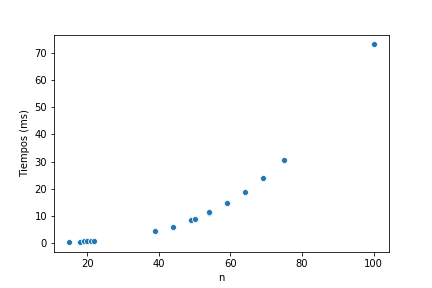
\includegraphics[width=1\textwidth]{images/savings/Ptiempos}
		\caption{\footnotesize Tiempo de acuerdo al tamaño de la entrada}
		\label{fig:savings-Ptiempos}
	\end{minipage}%
	\hspace{0.03\textwidth}
	\begin{minipage}{0.44\textwidth}
		\centering
		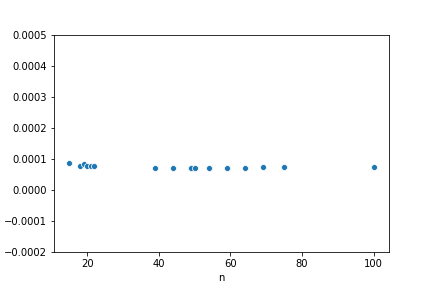
\includegraphics[width=1\textwidth]{images/savings/savingscte}
		\caption{\footnotesize Tiempo/complejidad de acuerdo al tamaño de la entrada}
		\label{fig:savings-Ptiempos-cte}
	\end{minipage}%
\end{figure}

\paragraph{}
En la figura \ref{fig:savings-Ptiempos} se observa que efectivamente crece a medida que crece $n$ y no parece haber una gran varianza entre instancias del mismo tamaño: esto indicaría que otro tipo de variaciones en la instancia no afecta en gran medida el tiempo de ejecución del algoritmo. En \ref{fig:savings-Ptiempos-cte} vemos graficada la curva que relaciona tiempos y complejidad. Al quedar una recta constante tenemos un gran indicio de que la complejidad es correcta o muy bien aproximada.
\paragraph{}
La otra cara de la experimentación fue ver que tan cerca están las soluciones de $savings$ del óptimo. Los óptimos de este data set son conocidos. Además, incluimos los casos donde savings no funciona tan bien. Esperamos que aunque pueda haber casos malos, en general no esté alejada del óptimo. 

\begin{figure}[H]
	\centering
	\begin{minipage}{0.50\textwidth}
	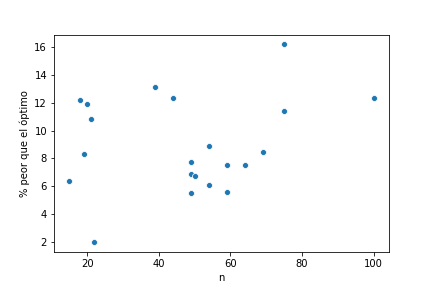
\includegraphics[width=1\textwidth]{images/savings/Pporcentaje}
	\caption{\footnotesize Porcentaje de acuerdo al tamaño de la entrada}
	\label{fig:savings-Pporcentaje}
	\end{minipage}
\end{figure}
\paragraph{} 
En \ref{fig:savings-Pporcentaje} calculamos cuanto aumenta en porcentaje la distancia de la solución de la heurística con respecto a la óptima. Vemos que los porcentajes varían siendo 2\% el caso más cercano al óptimo y casi \%16 el peor. Observamos que no parece depender de $n$: esto sí que depende del tipo de instancia, de como se formen las rutas y si la forma en que las crea savings es parecida a la del óptimo o no.
